% Created 2021-04-19 Mon 15:13
% Intended LaTeX compiler: pdflatex
\documentclass{article}
\usepackage[utf8]{inputenc}
\usepackage[T1]{fontenc}
\usepackage{graphicx}
\usepackage{grffile}
\usepackage{longtable}
\usepackage{wrapfig}
\usepackage{rotating}
\usepackage[normalem]{ulem}
\usepackage{amsmath}
\usepackage{textcomp}
\usepackage{amssymb}
\usepackage{capt-of}
\usepackage{hyperref}
\bibliographystyle{plain}
\author{Andrej Glavic, Yuanxi Liu 20688855, Rachel Morton 20925026,\\ Wasam Syed 20746474, Amy Wang}
\date{\today}
\title{363 Final Report: Stroop test}
\hypersetup{
 pdfauthor={Andrej Glavic, Yuanxi Liu 20688855, Rachel Morton 20925026,\\ Wasam Syed 20746474, Amy Wang},
 pdftitle={363 Final Report: Stroop test},
 pdfkeywords={},
 pdfsubject={},
 pdfcreator={Emacs 26.3 (Org mode 9.2.6)}, 
 pdflang={English}}
\begin{document}

\maketitle
\tableofcontents


\section{Introduction}
\label{sec:orgcbaed77}
John Ridley Stroop published the groundbreaking, "Studies of interference in serial verbal ractions" in the Journal of Experimental Psychology in 1935 \cite{Stroop1935}. Ever since, psychology students worldwide learn about the "Stroop effect", where incongruent stimuli take longer to process than do congruent stimuli. Even though Stroop wasn't the first to publish this effect, his experiments were foundational; his original study is one of the most-cited papers in the history of experimental psychology \cite{MacLeod1991Stroop}.

In one part of Stroop's classic study, participants had to say the ink colour of the printed word rather than read the word. For instance, if the word 'RED' was printed in purple ink, they were to say, "purple" and not "red". Stroop noticed that subjects took significantly longer to complete this colour naming task than one where they just had to name the colour of coloured squares. This difference in response time, or processing speed, is what is known as the Stroop effect.

\section{Methods}
\label{sec:orgd26a65a}
There have been many variations on Stroop's experiment over the years. Since key presses are easier to time than a person reading aloud, we chose to go with a "manual" Stroop task where reaction time is measured by how long it takes a participant to press a certain key on a keyboard after being shown the stimuli on the computer screen. We used the psychopy library in python to program the experiment \cite{Peirce2019Psychopy} and followed the example shown in the demo Stroop task at psytoolkit.org \cite{PsytoolkitStroopDemo}. We used Python to analyze the data and plot the results. 

\section{Results}
\label{sec:org9ed6915}

\subsection{Collect data into a dataframe:}
\label{sec:org69698fb}

In this section, we do the following 2 things. First, we import all the relevant libraries that we need for any code to run. Second, we iterate through all the csv files and merge them into one big pandas data frame called \texttt{data}.

\begin{verbatim}
#graphics :file "StroopPlot.png"
import pandas as pd
import os
import numpy as np
import matplotlib.pyplot as plt

files = os.listdir()

# Identify all csv files in the directory
csv_files = []
for file in files:
    if file[-4:] == ".csv":
	csv_files.append(file)
data = pd.DataFrame()
for file in csv_files:
    data = data.append(pd.read_csv(file))

pd.set_option('display.max_rows', None)
\end{verbatim}

\pagebreak
\setlength{\voffset}{-0.75in}

\subsection{Descriptive statistics}
\label{sec:org7a993fd}

(379, 4)

[\#\#] participants completed [\#\#] trials.


Congruent trials are where the colour word and the font colour match. Incongruent trials are where the ink colour is different than the colour word.


We calculated the Stroop effect as the average response time for correct, incongruent trials minus correct, congruent trials.

[t-test comparing the means of (correct) congruent vs (correct) incongruent trials.]



\subsection{Scatter Plot with Line of Best fit}
\label{sec:orga3b00b7}

The code below creates a scatter plot. This scatter plot illustrates the reaction time to each of 20 words displayed in a trial of the experiment. The x-axis corresponds to the 20 words in the test; the y-axis coresponds to response time in miliseconds. Only correct responses were plotted. We noticed that the response time did not seem to be affected by whether a participant was on their first, tenth, or last word, as times were nearly constant across the trial. However, when the word presented was congruent with the ink colour it appeared in, response times were faster. Conversely, participants reacted more slowly to words that were incongruent with their ink colour.

Here is the code we used to generate the scatter plot. On the next page we have the plot itself, which clearly differentiates between the congruent and incongruent responses and also shows a line of best fit for each congruency type.

\begin{verbatim}
#output graphics :file "StroopPlotScatter.jpg"

congruent_y = np.array([])
congruent_x = np.array([])
incongruent_y = np.array([])
incongruent_x = np.array([])

for i in data.iterrows():
    if i[1]['Correct']:
	if i[1]['Word'] == i[1]['Ink']:
	    congruent_x = np.append(congruent_x, i[0]+1)
	    congruent_y = np.append(congruent_y, i[1]['Response Time']*1000)
	else:
	    incongruent_x = np.append(incongruent_x, i[0]+1)
	    incongruent_y = np.append(incongruent_y, i[1]['Response Time']*1000)

plt.scatter(congruent_x, congruent_y)
m, b = np.polyfit(congruent_x, congruent_y, 1)
plt.plot(congruent_x, m*congruent_x + b)
scatter = plt.scatter(incongruent_x, incongruent_y)
m, b = np.polyfit(incongruent_x, incongruent_y, 1)
plt.plot(incongruent_x, m*incongruent_x + b)
plt.xticks(np.arange(1, 21, 1.0))
plt.legend(["Congruent stimulus", "Incongruent stimulus"])
plt.title("Stroop Responses Scatter Plot")
plt.xlabel("Trial Number in Experiment")
plt.ylabel("Response Time(ms)")
plt.savefig("StroopPlotScatter.jpg")
"StroopPlotScatter.jpg"

\end{verbatim}

\begin{center}
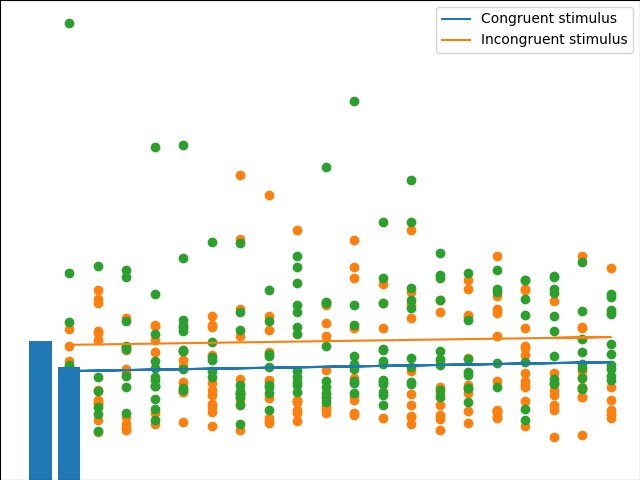
\includegraphics[width=.9\linewidth]{StroopPlotScatter.jpg}
\end{center}

\pagebreak


\subsection{Correct Stroop Responses and Calculated Average Response Time}
\label{sec:org93bdb50}

In this section, we calculate the average response time for both congruent and incongruent cases. We only consider instances where participants pressed the correct key. Below is the code we used to calculate the average response time. Following that we have the plot that illustrates the difference in the average response time.

\begin{verbatim}
#output graphics :file "StroopPlotAverage.jpg"
# Average Congruent vs Incongruent Time
congruent = np.array([])
incongruent = np.array([])
for i in data.iterrows():
    if i[1]['Correct']:
	if i[1]['Word'] == i[1]['Ink']:
	    congruent = np.append(congruent, i[1]['Response Time'])
	else:
	    incongruent = np.append(incongruent, i[1]['Response Time'])

width = 0.35
state = ('Congruent', 'Incongruent')
state_average = (np.average(congruent)*1000, np.average(incongruent)*1000)
fig, ax = plt.subplots()
rects = ax.bar(np.arange(2)+width, state_average, width, color='g')
ax.set_ylabel('Response Time (ms)')
ax.set_title('Response Time based on Congruency')
ax.set_xticks(np.arange(2)+width)
ax.set_xticklabels(('Congruent', 'Incongruent'))

plt.savefig("StroopPlotAverage.jpg")
"StroopPlotAverage.jpg"
\end{verbatim}

\begin{center}
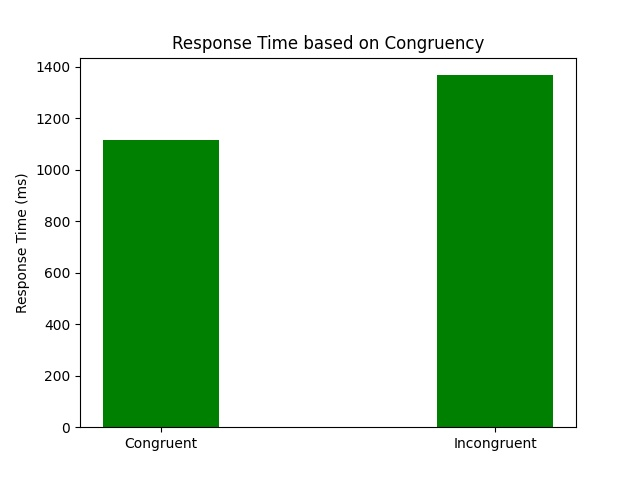
\includegraphics[width=.9\linewidth]{StroopPlotAverage.jpg}
\end{center}

\pagebreak


\subsection{Total Incorrect Stroop Responses Analysis}
\label{sec:org4ce073f}

The final graph we include here considers the incorrect responses. We found participants were much more likely to press an incorrect key in response to an incongruent word, when the word did not match the ink colour, than to a congruent word, when the word and ink colour matched. In our sample, there were 8 times as many incorrect keystrokes made for incongruent cases compared to congruent cases.

\begin{verbatim}
#output graphics :file "StroopPlotIncorrect.jpg"
congruent_wrong = 0
incongruent_wrong = 0
for i in data.iterrows():
    if not i[1]['Correct']:
	if i[1]['Word'] == i[1]['Ink']:
	    congruent_wrong+=1
	else:
	    incongruent_wrong+=1

width = 0.35
state = ('Congruent', 'Incongruent')
wrong_count  = (congruent_wrong, incongruent_wrong)
fig, ax = plt.subplots()
rects = ax.bar(np.arange(2)+width, wrong_count, width, color='r')
ax.set_ylabel('Total Incorrect Responses')
ax.set_title('Incorrect Responses Based on Congruency')
ax.set_xticks(np.arange(2)+width)
ax.set_xticklabels(('Congruent', 'Incongruent'))

plt.savefig("StroopPlotIncorrect.jpg")
"StroopPlotIncorrect.jpg"
\end{verbatim}

\begin{center}
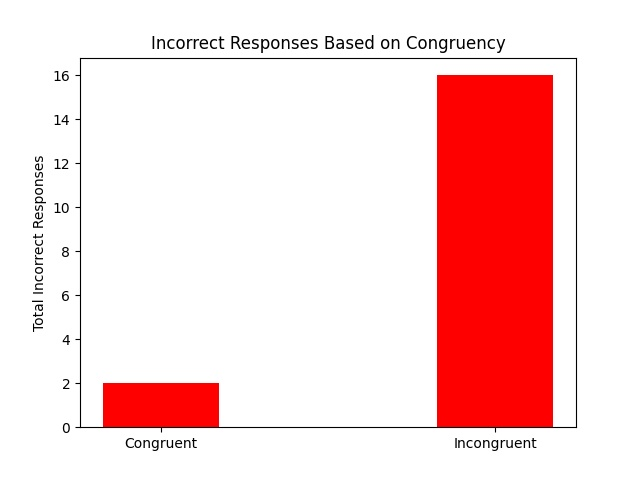
\includegraphics[width=.9\linewidth]{StroopPlotIncorrect.jpg}
\end{center}

\pagebreak

\section{Discussion and Conclusions}
\label{sec:orgd7e6639}

Our experiment takes less than two minutes to complete. It requires pressing the appropriate keyboard key rather than naming the colour aloud as Stroop did originally \cite{Stroop1935}. In our test, there are only 20 trials and a handful [\#\#?] of participants. For a more reliable measure of the Stroop effect you would want to have considerably more participants along with more trials.

However, even with our limited sample size, we saw clear evidence of a Stroop effect: words printed in an ink colour at odds with the word itself took longer to process and were more likely to result in mis-pressed keys than words that matched their ink colour. These differences in processing between congruent and incongruent stimuli are what make the Stroop effect such a fascinating, and popular, phenomenon to study.

\section{References}
\label{sec:org12ce34f}

\bibliography{finalReportBib}
\end{document}
